% \theoremstyle{definition}


본 연구의 연구 흐름에 대해 기술하는 장이다. motivation부터 연구를 이해하는데 필요한 배경 지식, 본 연구의 필요성 등이 논리적으로 함유되었다.

\section{NeRF and QRF}
% \subsection{NeRF and QRF}
% \textit{설명(삭제예정) : 컴퓨터 비전(상당히 대중적인 주제)의 문제로부터 양자머신러닝 모델의 잠재력을 어필하는 장이다.}

% 컴퓨터 비전 분야에서, 특정 객체에 대한 여러 사진을 Input으로 하여, 입력되지 않은 새로운 view에서의 객체의 형상을 모델링하는 task는 굉장히 중요한 문제이다. view synthesis라고 불리는 이 작업은, 기존에는 해당 객체를 포함한 공간(보통은 3D)의 정보를 모두 픽셀 단위로 저장하고, 이를 원하는 때에 알맞게 load하여 모델링하는 방식으로 이루어졌으나, 해상도가 높아짐에 따라 저장해야 하는 정보가 과도하게 많아진다는 문제가 있었다. 따라서 이를 효율화하기 위한 시도가 계속해서 존재했고, 대표적으로 NeRF(Neural Radiance Field)가 보다 효율적이고 안정적인 대체제가 되었다.
% NeRF 설명 ~~
% 그런데, NeRF 또한 이러이러한 단점이 존재했고, 이를 보완한 QRF(Quantum Radiance Field)가 대두되었다.

MLP(Multi-Layer Perceptron, 다층 퍼셉트론)는 머신러닝에서 사용되는 기본적인 모델로, 여러 분야에서 널리 사용되고 있다. 특히 컴퓨터비전 분야에서 중요한 작업인 3D view synthesis에서, NeRF(Neural Radiance Field)라는 기법이 MLP 모델을 사용하여 두드러진 성과를 보였다. NeRF가 3D view synthesis를 수행하는 방식은 다음과 같다. 먼저 3D 객체를 보는 방향 \( (\theta, \pi)  \in \mathbb{R}^2\)과 그 방향에 놓인 위치 좌표 $(x,y,z) \in \mathbb{R}^3$에 대한 정보가 주어졌을 때, MLP를 사용하여 $\text{color 정보 }(r,g,b) \in \mathbb{R}^3$ 를 예측한다. 이렇게 예측한 color값들은 volume rendering(이산 적분)을 통해, 특정 카메라 위치에서 바라본 이미지의 최종 color값을 예측하는 데 사용된다. 즉, 이산적인 2D view 이미지 데이터를 통해 학습하여, 연속적인 view에 대해서 이미지를 렌더링 할 수 있게 된다. 이러한 방법은 view에 대해 색상 값을 효과적으로 생성하면서도 낮은 저장 공간 요구와 빠른 추론 시간을 유지하기 때문에 많은 관심을 받았다.

 그러나 NeRF는 MLP 구조에 의존하고 있어 속도와 효율성 측면에서 한계가 있다. 최근 문헌에서는 NeRF의 머신러닝 과정을 양자컴퓨팅으로 대체하면 속도와 성능이 향상될 수 있다는 주장이 제기되었다. 이러한 제안은 QRF(Quantum Radiance Field) 연구에서 강조되며, NeRF 프레임워크에 양자 머신러닝을 통합함으로써 현재의 제약을 극복할 수 있는 잠재적 이점에 대해 논의하고 있다.

QRF는 NeRF에서의 ML 모델을 PQC(Parameterized Quantum Circuit) 모델로 대체한 것으로, 큰 차원의 데이터를 양자 데이터로 인코딩함에 따라 데이터의 규모를 축소하고, 이를 통해 resource와 연산 측면의 이득을 취하였다(고 주장한다). 그러나 QRF를 제안한 논문에서는 성능이 왜 개선되었는가에 대한 수학적 근거가 제시되지 않았다. 이에 우리는 궁극적으로 QRF가 실제로 작동하는지, 작동한다면 왜 좋은 결과를 나타내는지에 대해 의문을 갖고, NeRF와 QRF의 핵심인 ML과 QML 차원에서의 수학적인 비교 분석을 하게 되었다.

% 이에 우리는 이 방법론이 실제로 작동하는지, 작동하면 왜 좋은 결과를 나타내는지 수학적으로 분석하고자 하였다.
% 속도가 왜 빨라졌는지, 정확성이 왜 높아졌는지에
% ==> 우리가 이 연구를 시작하게 되었다. 먼저 얘는 ML, QML의 차이이기 때문에 ML, QML의 분석이 선행되었다.

% \subsection{ML and QML}\label{ss:ml and qml}
% 설명(삭제예정) : QRF로 설득한 QML의 잠재력을 가지고 ML과 QML의 공통점/차이점, QML의 필요성 등을 더 설명하는 장이다. 사실 3.1.1만 있으면 좀 부실해보여서 넣는 장이긴 함
% QML의 연구가치, 적용 가능해 보이는 분야들 -> 진짜 motivation이 될 수 있을 법한 내용들

% 이처럼
% 양자 머신러닝은 기존 머신러닝의 한계를 극복하는 데 효용이 있을 것으로 기대되어 활발히 연구 중인 주제이며, ML과 QML의 대표적인 공통점과 차이점은 다음과 같다.

% 공통점으로는, 전체 구조적으로 동일한 양상을 띈다는 것이 있다. ML과 QML 모두 데이터를 Encoding하고, 문제에 맞게 구성된 모델을 통해 output을 내놓는다. 이렇게 얻은 output을 통해 미리 정의된 cost function의 출력값을 계산하고, 계산된 cost 값을 최소화하도록 학습이 진행된다.

% ML과 QML의 가장 큰 차이점은, QML 모델은 데이터 인코딩부터 output 값을 생성하는데까지의 과정이 양자 컴퓨터 상의 양자 알고리즘으로 이루어진다는 것이다. QML 모델은 후술할 여러 방법들을 통해 가지고 있던 기존의 데이터를 중첩시킨 양자 데이터로 변환하고, 양자 회로로 이루어진 Ansatz를 통해 output을 내놓게 된다. 대부분의 QML에서, 이후의 optimize 과정은 고전 ML과 동일하다.

% QML은 양자 컴퓨터에서 작동하는 양자 알고리즘의 이점을 활용하고자 하며, 다양한 방법을 통해 다양한 분야로 적용하려 하는 시도들이 행해지고 있다. 이에 양자 머신러닝의 근간이 되는 양자컴퓨팅의 수학적 이론부터, 양자 머신러닝이 행해지는 방법과 원리를 이해하고 이를 분석해보았다.


%#########################################################
% 3.3 Quantum Machine Learning
%
% Author : SEHYUN YUK
% Last Update: 2024.12.08
%
%##########################################################
\section{Implementations and Experiments} \label{qml:comparision}

 이 절에서는 우리의 본래 목적인, QRF에서 사용된 QML의 세부 요소를 설명한다. 또한 두 가지 문제에 대해 ML과 QML 모델을 각각 구현하여 실제 ML과 QML의 결과값을 비교 분석해보고자 한다.


% 이 절은 우리의 본래 목적인 실험적으로 드러나는 QML과 ML의 차이를 수학적으로 보이는 절이다.
공평한 비교를 위해 똑같은 데이터를 사용하고, 똑같은 파라미터의 개수를 사용하였을 때, 특정함수를 추정하는 Task에서의 성능차이를 보이고자 하였다. 먼저 QRF논문에서 사용된 2d image를 reconstruction 하는 Task에서 작동방식을 확인하고, 이를 더 확실하게 검증하기 위해 1차원 함수를 추정하는 Task에서 또한 검증을 추가적으로 진행하였다.
\begin{itemize}
    \item \textbf{2d image reconstruction} :

        본 태스크는 xy 좌표를 입력으로 받아 RGB 값의 3차원을 예측하는 문제이다. 모델은 각 좌표 \((x, y)\)에 대해 색상 벡터 \((r, g, b)\)를 예측하며, 예측된 색상과 실제 색상 간의 손실을 계산하여 학습을 진행한다. 이를 수식으로 표현하면 다음과 같다.

            \[
            \text{Input}: \mathbf{p} = (x, y) \in \mathbb{R}^2
            \]

            \[
            \text{Prediction}: \hat{\mathbf{c}} = (\hat{r}, \hat{g}, \hat{b}) = f(\mathbf{p}; \theta)
            \]

            \[
            \text{Loss Function}: \mathcal{L}(\theta) = \frac{1}{N} \sum_{i=1}^{N} \| \hat{\mathbf{c}}_i - \mathbf{c}_i \|_2^2
            \]




            여기서 \(f\)는 모델 함수, \(\theta\)는 모델의 파라미터, \(N\)은 데이터 샘플의 수를 나타낸다. 모델은 손실 함수를 최소화하도록 파라미터 \(\theta\)를 최적화하여 예측된 RGB 값이 실제 값과 잘 일치하도록 학습된다. 여기서 ML과 QML의 차이는 모델과 데이터 인코딩에서만 차이나는데, 각각 다음과 같이 진행된다.


              \begin{table}[ht]
                    \centering
                    \begin{tabular}{ l||p{5.5cm}||p{5.5cm}}
                    \Xhline{3\arrayrulewidth}
                    \textbf{Item} & \textbf{MLP} & \textbf{QML} \\
                    \hline
                    Data Encoding & $(x,y) \in \mathbb{R}^2$을 $[-1 ,1]$ 사이로 정규화 하였다.    &
                    Angle Encoding을 사용하였다.$(x,y) \in \mathbb{R}^2$을 $[-1 ,1]$ 사이로 정규화한 이후 이 두 값을 3 개의 qubit 중 두개의 quibt에 RX gate에 $\theta_x ,\theta_y  $들을 각각 $ [-\pi ,\pi]$ 값 사이에 위치하도록 정규화하여  Angle encdoing 하였다.
                     \\
                    \hline
                    Model & MLP 모델을 사용하였으며, 입력에이어 1개 , 히든 레이어 1개 ,출력 레이어 1개로 구성하였으며, activation function은 RELU를 사용하였다. &
                    QRF에서 사용된 PQC 모델과 동일하도록 사용하였다. 총 3개의 qubit을 사용하였고, $ \prod_{0}^{2} RY_i(\theta)CX_i$ 의 gate를 3번 반복함으로써 3층의 레이어의 효과가 나타나도록 구현하였다. 이를 시각화면 다음과 같다.\labelcref{fig:2d-image}
                     \\
                    \Xhline{3\arrayrulewidth}
                    \end{tabular}
                    \caption{MLP와 QML의 비교}
                    \label{tab:mlp_qml_comparison}
                \end{table}

                % \clearpage
                \begin{figure}[h]
                    \centering
                    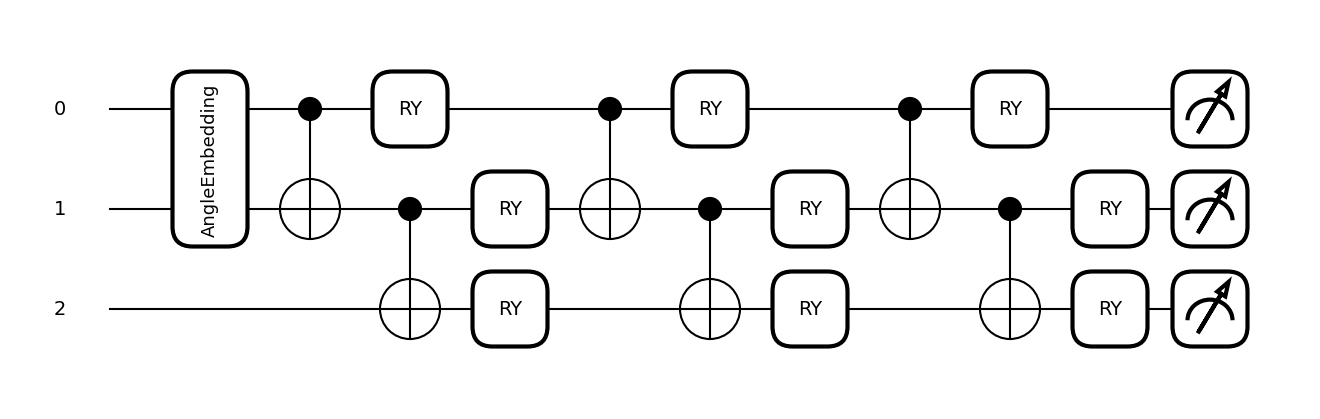
\includegraphics[width=0.8\textwidth]{figs/pqc_2d}\
                \caption{2-d image quantum circuit 구조}
                \label{fig:2d-image}
                \end{figure}

                이러한 모델은, 우리는 사진 3장(256x256)에 대하여, reconstruction error를 PSNR metric를 사용하여 학습된 성능을 평가하였다. PSNR의 수식은 다음과 같이 정의 된다.이는 높은 PSNR이 더 잘 reconstruction함을 뜻한다.

                \[
                    \text{PSNR} = 10 \cdot \log_{10}\left(\frac{\text{MAX}_I^2}{\text{MSE}}\right)
                    \]

                이와 같은 방법으로, 여러 layer별로 성능차이를 비교해보았으며, 결과는 다음과 같이 나타났다.

                \begin{table}[ht]
                    \centering
                    \begin{tabular}{c|ccc}
                    \Xhline{3\arrayrulewidth}
                    \multirow{2}{*}{Layers} & \multicolumn{3}{c}{PSNR (dB)} \\
                    \cline{2-4}
                    & Image 1 & Image 2 & Image 3 \\
                    \hline
                    MLP (3 layers) & 15.826 & 16.913 & 15.884 \\
                    MLP (4 layers) & 15.816 & 17.049 & 16.328 \\
                    MLP (5 layers) & 15.811 & 16.606 & 16.306 \\
                    \hline
                    PQC (3 layers) & 14.503 & 16.269 & 15.470 \\
                    PQC (4 layers) & 15.624 & 16.464 & 15.471 \\
                    PQC (5 layers) & 4.484 & 6.912 & 8.786 \\

                    \Xhline{3\arrayrulewidth}
                    \end{tabular}
                    \caption{PSNR comparison between MLP and QML models across different layer configurations}
                    \label{tab:psnr_comparison}
                \end{table}

        \item \textbf{1-d function estimation} :
본 태스크는 1차원 입력 x를 받아 스칼라 값 y를 예측하는 문제이다. 모델은 입력 x에 대해 출력 y를 예측하며, 예측된 값과 실제 값 간의 손실을 계산하여 학습을 진행한다. 이를 수식으로 표현하면 다음과 같다:

\[
\text{Input}: x \in \mathbb{R}
\]

\[
\text{Prediction}: \hat{y} = f(x; \theta)
\]

\[
\text{Loss Function}: \mathcal{L}(\theta) = \frac{1}{N} \sum_{i=1}^{N} (\hat{y}_i - y_i)^2
\]

여기서 \(f\)는 모델 함수, \(\theta\)는 모델의 파라미터, \(N\)은 데이터 샘플의 수를 나타낸다. 모델은 손실 함수를 최소화하도록 파라미터 \(\theta\)를 최적화하여 예측된 값이 실제 값과 잘 일치하도록 학습된다. ML과 QML의 차이는 모델과 데이터 인코딩에서만 차이나는데, 각각 다음과 같이 진행된다.


\begin{table}[ht]
    \centering
    \begin{tabular}{ l||p{5.5cm}||p{5.5cm}}
    \Xhline{3\arrayrulewidth}
    \textbf{Item} & \textbf{MLP} & \textbf{QML} \\
    \hline
    Data Encoding & $x \in \mathbb{R}$을 $[-1, 1]$ 사이로 정규화하였다. &
    Angle Encoding을 사용하였다. $x \in \mathbb{R}$을 $[-1, 1]$ 사이로 정규화한 이후, 이 값을 2개의 qubit 중 첫 번째 qubit의 RX gate에 $\theta_x$를 $[-\pi, \pi]$ 값 사이에 위치하도록 정규화하여 Angle encoding 하였다. \\
    \hline
    Model & MLP 모델을 사용하였으며, 입력 레이어 1개, 히든 레이어 1개, 출력 레이어 1개로 구성하였으며, activation function은 RELU를 사용하였다. &
    2개의 qubit을 사용하였고, $\prod_{0}^{1} RY_i(\theta)CX_i$의 gate를 3번 반복함으로써 3층의 레이어의 효과가 나타나도록 구현하였다.이를 다음과 같이 시각화하였다.\labelcref{fig:1d-image} \\
    \Xhline{3\arrayrulewidth}
    \end{tabular}
    \caption{MLP와 QML의 비교}
    \label{tab:mlp_qml_comparison_1d}
\end{table}

\begin{figure}[h]
    \centering
    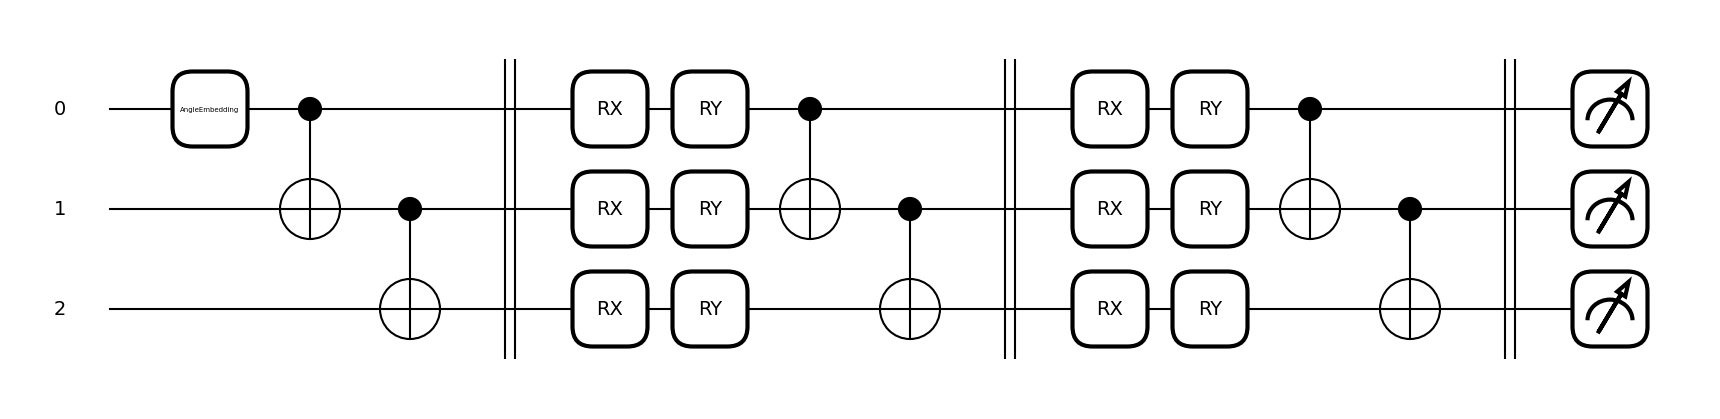
\includegraphics[width=0.8\textwidth]{figs/pqc_1d}\
\caption{1-d function estimation quantum circuit 구조}
\label{fig:1d-image}
\end{figure}
\end{itemize}
\clearpage

이 실험또한 마찬가지로, 여러 레이어의 개수로 실험하였고, 다양성을 위해 3 개의 함수에서 MSE  결과를 측정하였다.

\begin{table}[ht]
    \centering
    \begin{tabular}{c|ccc}
    \Xhline{3\arrayrulewidth}
    \multirow{2}{*}{Layers} & \multicolumn{3}{c}{MSE} \\
    \cline{2-4}
    & $sin(x)$  & $tanh(x)$ & $x$ \\
    \hline
    MLP (3 layers) & 0.0 & 0.0 & 0.0 \\
    MLP (4 layers) & 0.0 & 0.0 & 0.0 \\
    MLP (5 layers) & 0.0 & 0.0 & 0.0 \\
    \hline
    PQC (3 layers) & 0.0 & 0.0 & 0.003 \\
    PQC (4 layers) & 0.0 & 0.0 & 0.003 \\
    PQC (5 layers) & 0.0 & 0.0 & 0.003 \\
    \Xhline{3\arrayrulewidth}
    \end{tabular}
    \caption{MSEcomparison between MLP and QML models across different layer configurations}
    \label{tab:mse_comparison}
\end{table}




\section{Limitations of QML: Constraint of Nonlinearity}

3.3절에서 살펴본 결과, QML이 2d, 1d에서 잘 작동하지 않는 것을 확인하였다. 이에 대한 이유를 quantum circuit의 비선형성의 부족으로 유추하였다. 이를 수학적으로 분석하기 위해, QML의 circuit 구조에 따라, 입력에서 출력까지 나오게 되는 과정을 수식화하였다. \labelcref{fig:1d-image} 와 \labelcref{fig:2d-image}들은 3 qubit cricuit 이므로 gate들의 연산을 모두 $8x8$ 행렬로 나타낼 수 있다. 이러한 행렬의 곱셈연산과 마지막 observable 과정 $ \langle \psi | O | \psi \rangle$ 을 거치면, 마지막 출력 값을 입력에 대한 식으로 표현할 수 있다.  sympy 라이브러리를 통해 식 간략화 및 계산 전개등을 수행하였고 최종식을 도출하였다. 이 식이 정당성에 대한 검증은 실제모델의 값과 비교해봄으로써 확인하였다.

 \labelcref{fig:1d-image} 의 출력을 행렬연산을 통해 도출한 최종값을 수식으로 표현하면 다음과 같이 표현된다.

\begin{equation*}
    y_1  = c_1\cos{\left(x_{1} \right)} - c_2\cos{\left(x_{2} \right)} - c_3\cos{\left(x_{1} - x_{2} \right)} - c_4\cos{\left(x_{1} + x_{2} \right)}
\end{equation*}


\begin{equation*}
y_2  = - c_4\cos{\left(x_{1} \right)} + c_5\cos{\left(x_{2} \right)} - c_6\cos{\left(x_{1} - x_{2} \right)} - c_7\cos{\left(x_{1} + x_{2} \right)} - c_8
\end{equation*}

\begin{equation*}
   y_3 =  -c_9 \cos{\left(x_{1} \right)} + c_{11} \cos{\left(x_{2} \right)} - c_{12} \cos{\left(x_{1} - x_{2} \right)} - c_{13} \cos{\left(x_{1} + x_{2} \right)} - c_{14}
\end{equation*}


여기서 $ c_i $ 들은 PQC의 파라미터에 따라 변하는 값들이며, 매우 복잡한 파라미터값들의 곱 연산을 통해 계산된다. 그러나 최종적으로 파라미터 값이 결정되면 이 값들은 고정되며, $ y_1 ,y_2 , y_3 $ 값들은  $\cos(x_1)$과 $\cos(x_2)$들과 $c_i$ 값들의 linear combination으로 이루어진다. 이를 통해 출력이 선형적이며, 제한된 표현력을 가지고 있음을 관찰하였다.

\clearpage

\labelcref{fig:2d-image}에서 의 출력또한 행렬연산을 통해 최종값을 수식을 도출하였고 이를 수식으로 표현하면 다음과 같다.

\begin{equation*}
 y = - c_1 \sin{\left(x_{1} \right)} - c_2 \cos{\left(x_{1} \right)} + c_3
\end{equation*}

여기서 또한 $c_i$ 값들이 고정되면  $sin(x)$ 와 $cos(x)$ 형태의 linear combination으로 표현되며, 이러한 식은 삼각함수 근사에서만 높은 성능을 보였던 것을 잘 설명해준다. 이러한 선형성은 $\sin(x)$와 $\cos(x)$ 에 대해서만 표현되는 제한적인 표현력을 보여주며, 다양한 함수를 근사하기 위해서는 반드시 비선형성이 필요하다는 것을 시사한다.

